\chapter{Recovering the Cost Matrix}
\label{ch:results}
In this Chapter, we will use Algorithm \ref{alg:1} to find the cost matrix of the simulations. As described in Section~\ref{sec:algimp}, $R(c) = \mathbbm{1}_U$ and $U = [0, M_c]^3$ are used. For all future results, we choose $\gamma = \varepsilon = 1$. Note that we will only recover $c$ up to a constant scaling, and not $c$ itself; we will recover $c/\varepsilon$. Therefore, the value of $\varepsilon$ we choose is not important for the results, as long as a consistent value of $\varepsilon$ is used. Furthermore, a value of $M_c = 10$ is chosen, in order to have enough accuracy and still be computationally efficient enough to run multiple cases. 

\section{Reference Cases}
\label{sec:refs}
To help interpret the results of FLAMINGO data, a few reference cases will be calculated. To better see differences in the heat map of the acquired cost matrix, we manually set all entries that were equal to $M_c$, equal to the highest entry of $c$ that is not equal to $M_c$. In some cases, this scaling will not be performed as this will result in a uniform heat map. These cases will be mentioned mention separately. All reference cases are simulated with one million particles. In this section, some initial reference cases were tested for a certain number of boxes. More reference cases are described in Appendix~\ref{sec:apprefs}.

\subsection{Linear Motion}
As a first reference case, consider particles with linear motion and constant velocity. For the simulation, a box size of $100$ (arbitrary units) was used. All particles started in the box $[0, 50]^3$, and moved with the same velocity towards $[50,100]^3$. All particles have an equal $x$-, $y$- and $z$-velocity. \par 
For the case $n=2$, where each axis is divided into $2$ segments, we have $8$ boxes in total. Here, a low cost for $c_{07}$ is expected, and a high cost everywhere else. This low cost at $c_{07}$ is because all particles are going from box $0$ (which is $[0, 50]^3$) to box $7$ (which is $[50, 100]^3$), and no particles are going anywhere else. As we can see in Figure~\ref{fig:uniformlin}, in the case $n=2$ we have indeed a very low cost in $c_{07}$ and a high cost everywhere else. Note that in Figure~\ref{fig:uniformlin}, and all following heat maps of the cost matrix, the $y$-axis is the $i$ in $c_{ij}$, where the particles came from, and the $x$-axis is the $j$ in $c_{ij}$, where the particles are moving to. Note that the $n=2$ case in Figure~\ref{fig:uniformlin} is not scaled as described above in Section~\ref{sec:refs}, as this scaling would result in a uniform heat map.\par 

\begin{figure}[p]
	\centering 
	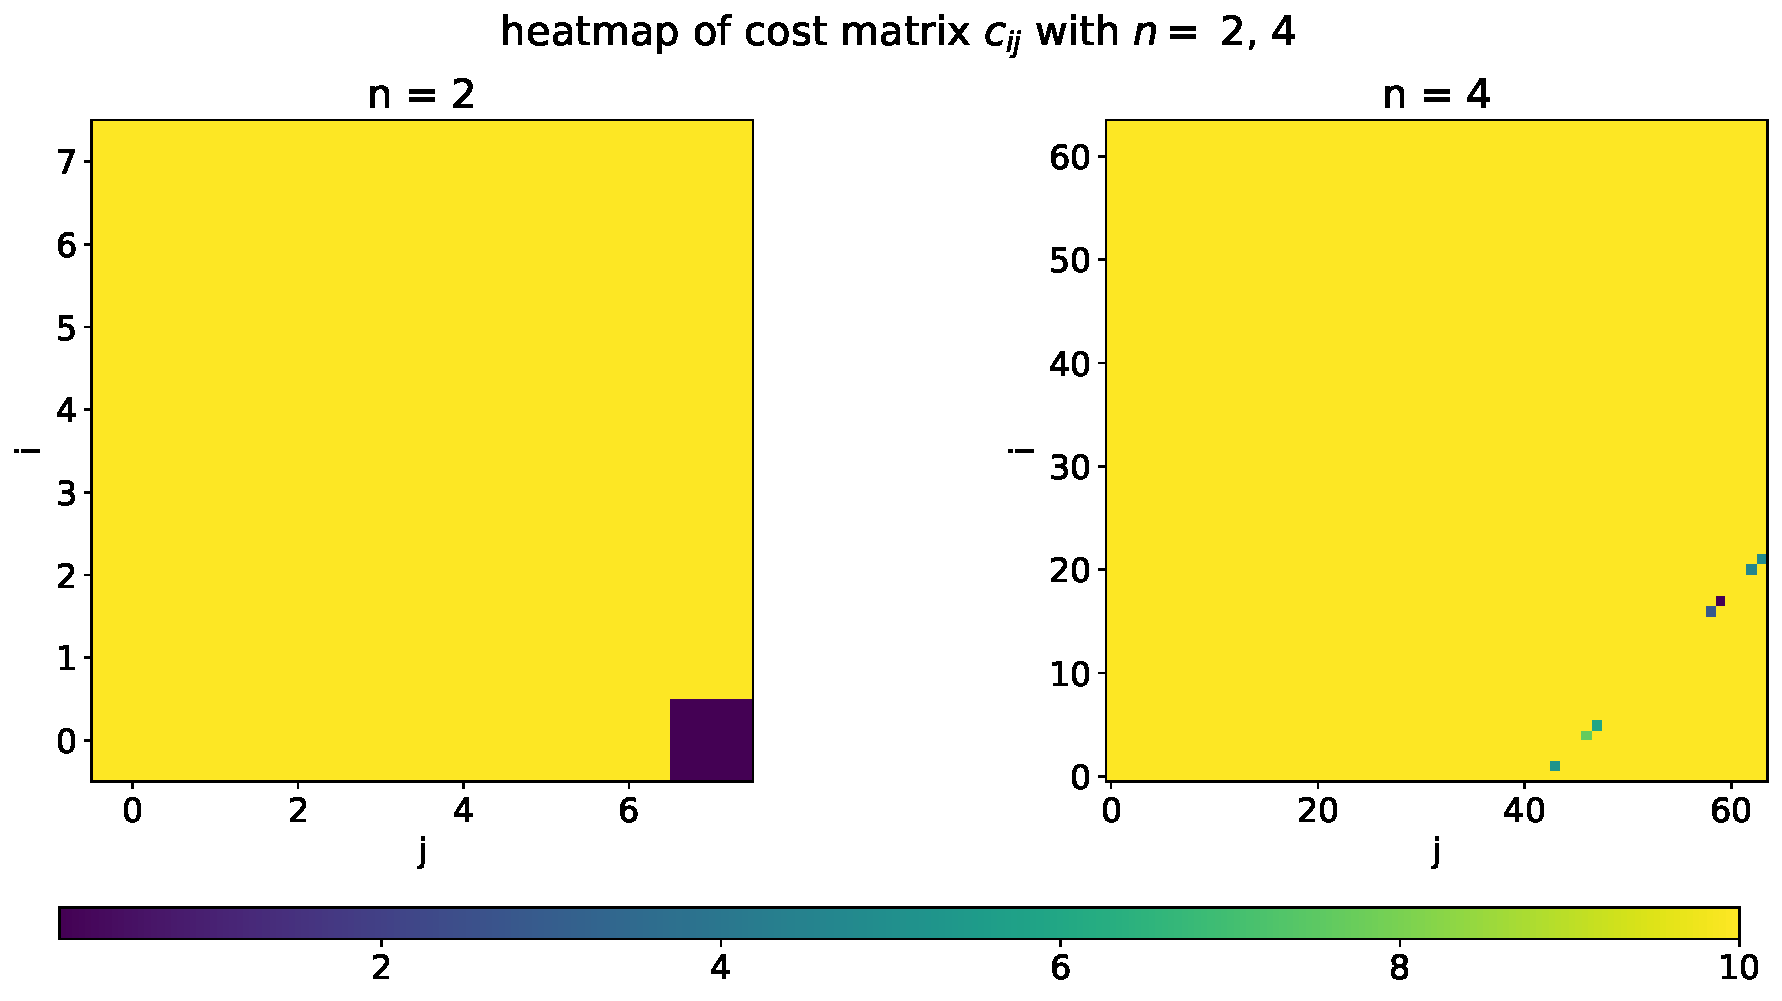
\includegraphics[width=\textwidth]{./images/uniform_v_ma_ncombined-n4-new.pdf}
	\caption{Heat map of the cost matrix for uniform linear motion from $[0, 50]^3$ to $[50, 100]^3$, for $n = 2$ (left) and $n = 4$ (right), as retrieved from Algorithm~\ref{alg:1}. The $n=2$ case is not scaled as described in Section~\ref{sec:refs}. }
	\label{fig:uniformlin}
\end{figure}
\begin{figure}[p]
	\centering 
	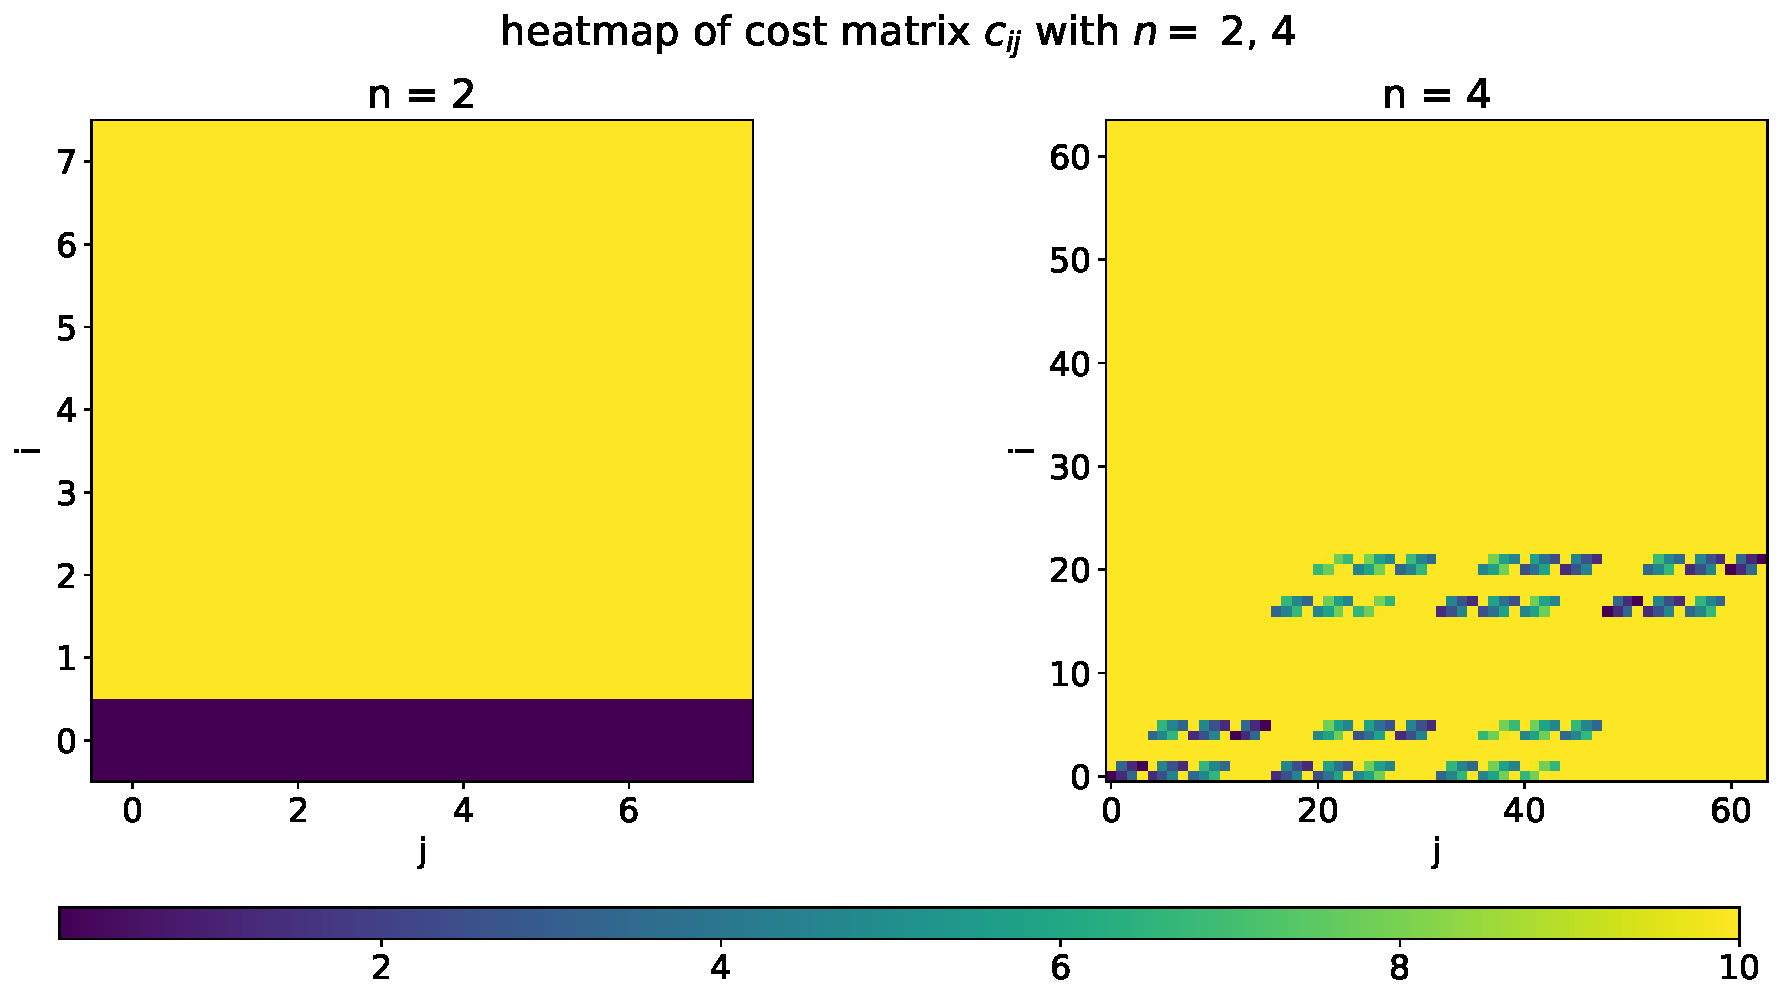
\includegraphics[width=\textwidth]{./images/nonuniform_v_ma_ncombined-n4-new.pdf}
	\caption{Heat map of the cost matrix for non-uniform linear motion from $[0, 50]^3$, for $n = 2$ (left) and $n=4$ (right), as retrieved from Algorithm~\ref{alg:1}. The $n=2$ case is not scaled as described in Section~\ref{sec:refs}. }
	\label{fig:nonuniformlin}
\end{figure}

Also for $n=4$ we can see a structure we would expect - there is some motion from $[0, 50]^3$, which is now divided into multiple boxes with low box number, to $[50, 100]^3$, which is divided into boxes with a higher box number. \par 
Note that, in general, the $n=2$ case is not the averaged $n=4$ case, due to the way the boxes are numbered, as box $0$ does not split into box $0, 1, 2$ and $3$. \par 
The same can be done for non-uniform motion. Let all the particles, again, go from $[0, 50]^3$, but add a non-linearity in the velocity. Now, the particles have $x$-, $y$- and $z$-velocities, which are not necessarily the same. Thus, particles can end up anywhere in $[0, 100]^3$. Again, it is expected that $\pihat_{ij}$ is high for a low $i$ (going from $[0, 50]^3$), and $\pihat_{ij}$ can be high for any $j$, since the particles can end up anywhere in $[0,100]^3$. Hence, we can expect that $c_{ij}$ is low for low $i$. Furthermore, more low-cost entries of $c$ are expected than in the uniform case. After all, all the particles did not move the same amount in $x$, so they might have gone to different boxes. \par 
As we can see in Figure~\ref{fig:nonuniformlin}, in the case $n=2$ we have indeed a very low cost moving away from box $0$ (where all particles started), and a high cost everywhere else, which is what was expected. Note that the $n=2$ case in Figure~\ref{fig:nonuniformlin} is, again, not scaled as described in Section~\ref{sec:refs}, as this scaling would result in a uniform heat map.\par 
For $n = 4$ in Figure~\ref{fig:nonuniformlin}, we can see more structure, but notably still only low cost for low values of $i$. The structure that can be seen is indeed a structure we would expect; there is some motion from the boxes in $[0, 50]^3$ to most other boxes. \par 
Thus, we can see that there are clear differences in the shape of the cost matrix with particle movements of constant and non-uniform velocity, which can be useful to determine structures in the cost matrix from the simulations. 

\subsection{Voids}
\label{sec:voids}
Forms of motion that are more common in the evolution of the Universe, are expansion and collapse \citep{planelles2014}. Let us consider (uniform and non-uniform) expansion, which tends to happen in voids. Again, a box size of $100$ (arbitrary units) is used. All data points start in a cube centered at $(50, 50, 50)$ with sides of $50$, and particles can move towards the whole box. \par 
We start by considering uniform expansion along three (spatial) dimensions. A scale factor can be calculated by using the initial and final radius, while scaling the points accordingly. Because we are considering particle to expand from a certain point, we can expect a symmetric cost matrix. Note that the axis of symmetry does not necessarily have to be the line $y = x$ (from $(0,0)$ to $(n^3, n^3)$), as the center of expansion is not necessarily in the center of a box, or in box $n^3/2$. Furthermore, for the $n=2$ case, no motion between boxes can be expected, as there is no side-to-side motion. This is indeed what we can see in Figure~\ref{fig:uniformexp}; we see a diagonal cost matrix. Note that the one square that has the same colour as the background, $c_{55}$, is due to the scaling as described in Section~\ref{sec:refs} and this is not inherent to the system. \par 
The case for $n=4$, which can also be seen in Figure~\ref{fig:uniformexp}, looks a bit more interesting. We can see that the cost seems to be almost symmetric in an almost diagonal line, which is what is to be expected for expansion. If we count the boxes, we can see that boxes $21, 22, 25, 26, 37, 38, 41$ and $42$ are indeed in the center of the (full) box. Movement from those boxes outwards, which is where we can see a lower cost in Figure~\ref{fig:uniformexp}, is indeed what we would expect.

\begin{figure}[p]
	\centering 
	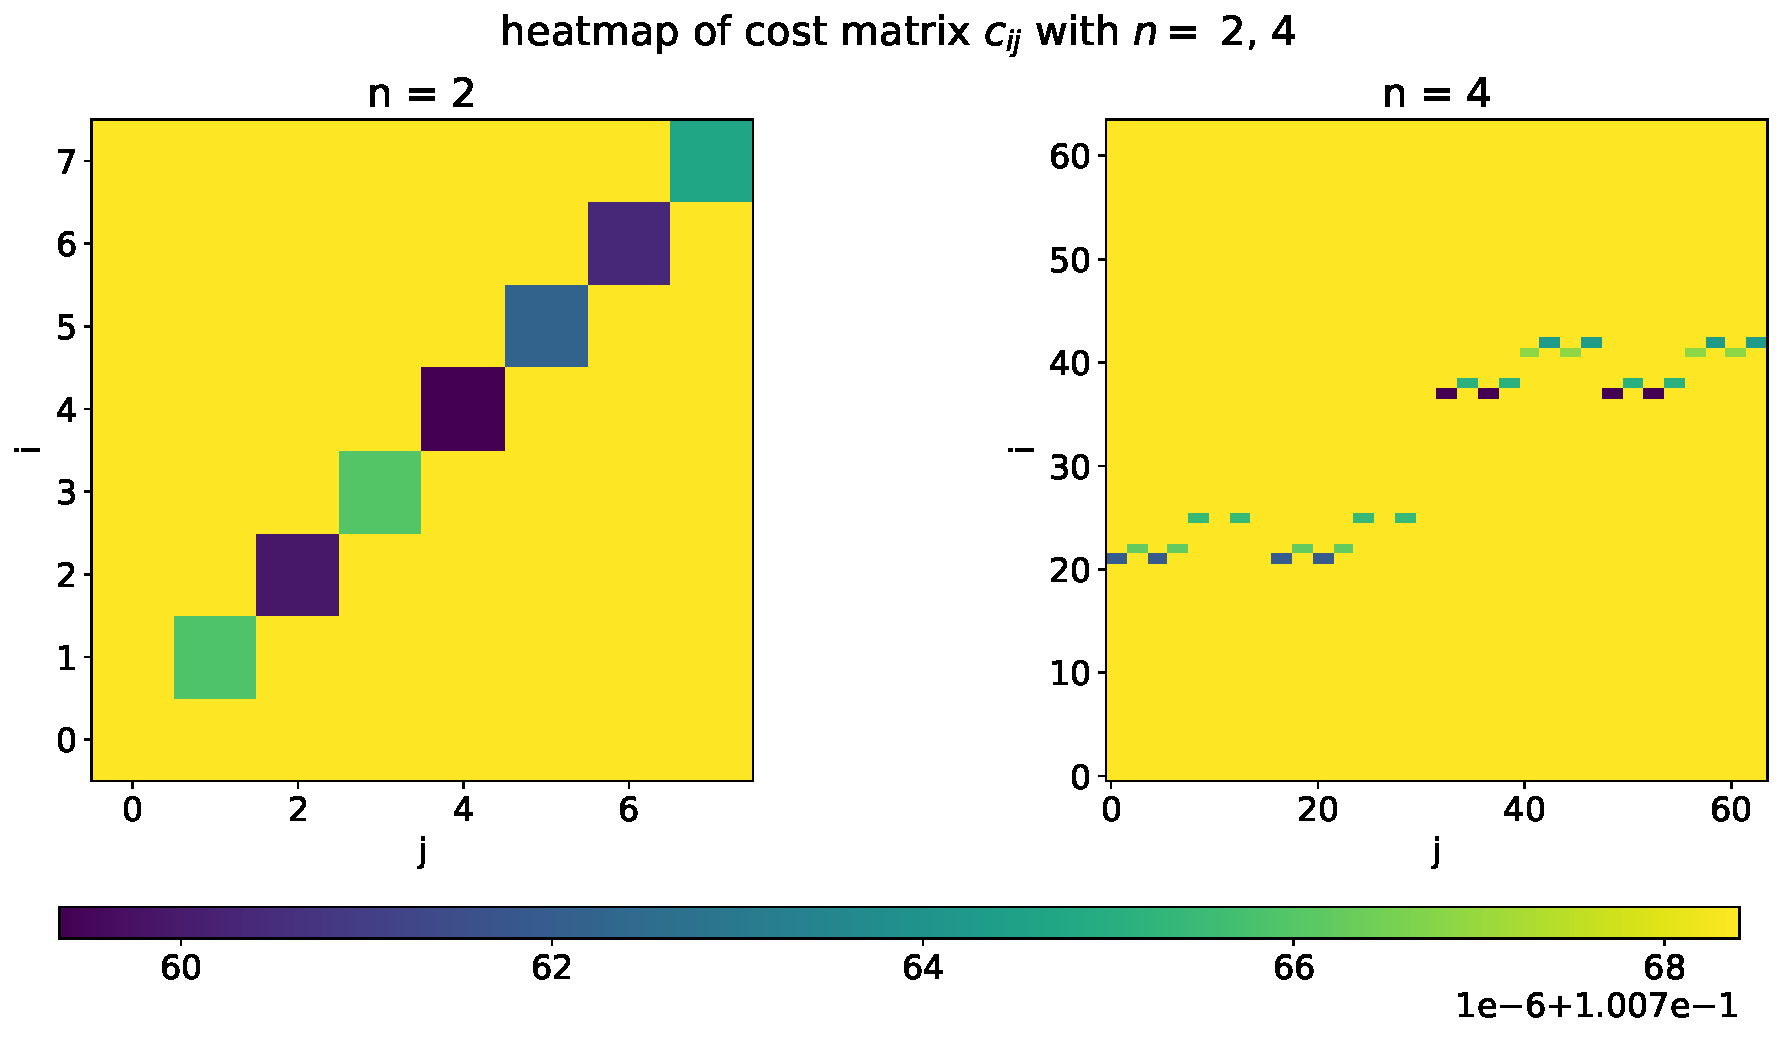
\includegraphics[width=\textwidth]{./images/uniform_expansion_ma_ncombined-n4-new.pdf}
	\caption{Heat map of the cost matrix for uniform expansion, for $n = 2$ (left) and $n = 4$ (right), as retrieved from Algorithm~\ref{alg:1}.}
	\label{fig:uniformexp}
\end{figure}
\begin{figure}[p]
	\centering 
	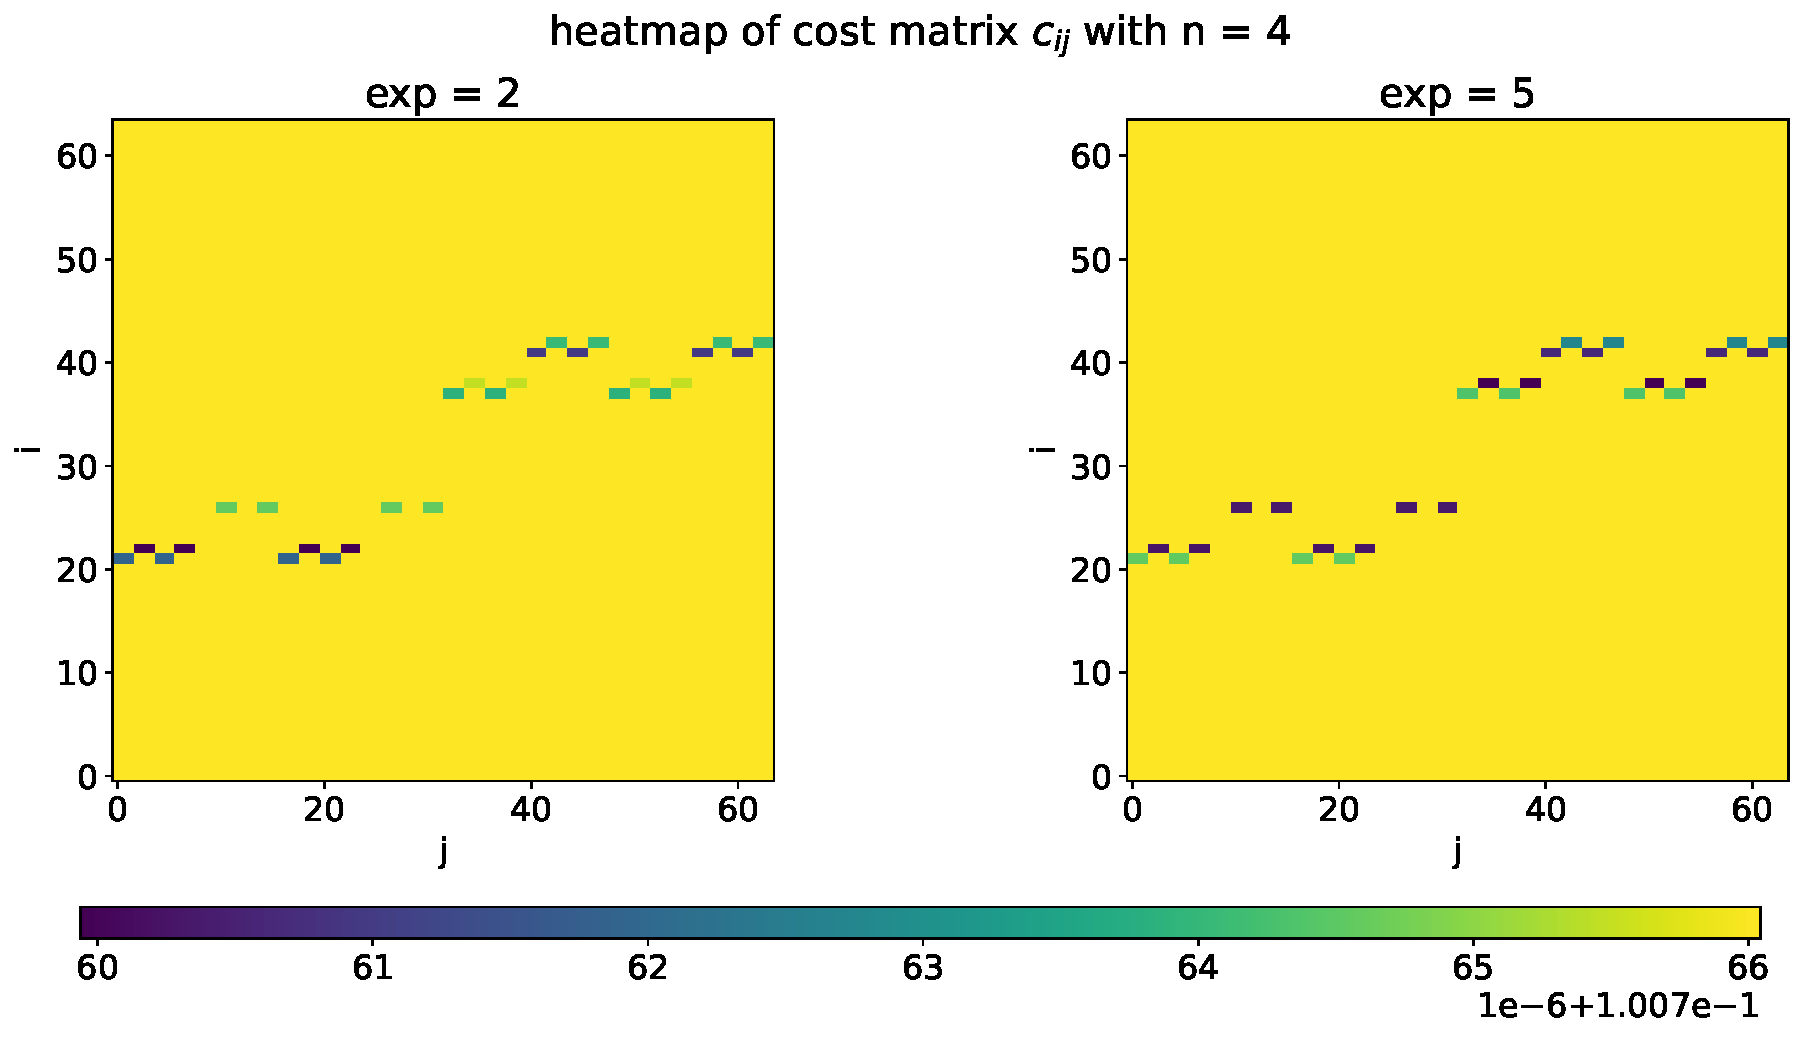
\includegraphics[width=\textwidth]{./images/nonuniform_expansion_ma_n4_c-combined-exp[2, 5]-new.pdf}
	\caption{Heat map of the cost matrix for non-uniform expansion, for both \lstinline|exp| $= 2$ (left) and \lstinline|exp| $=5$ (right), for $n = 4$, as retrieved from Algorithm~\ref{alg:1}. }
	\label{fig:nonuniformexpn4}
\end{figure}


Now, let us look at non-uniform expansion, again along three spatial dimensions. Here, one should choose how to simulate the non-uniformity. Physically, it makes the most sense to have accelerating expansion from a certain central point, in our case taken as the center point of our begin cube of points, which is the middle of the full box. The points will have an exponential velocity, depending on the distance from the center. This non-uniformity is implementing by using a parameter \lstinline|exp|.  When points are expanding from the initial sphere to a final, larger sphere, \lstinline|exp| controls the distribution of the radial displacement of each particle. Specifically, the initial distance of each particle from the center of expansion is calculated, and then normalized. This gives a set of normalized distances, \lstinline|normalized_distances|. These normalized distances then undergo a transformation where each element is raised to the power of \lstinline|exp|, \lstinline|scaled_normalized_distances = normalized_distances ** exp|. \par  
Note that if \lstinline|exp| $=1$, the expansion is uniform. For \lstinline|exp| $>1$, there is proportionally smaller displacement for particles closer to the center of expansion, than for particles that started far from the center of expansion, leading to a relatively dense distribution of particles near the center, and a relative thin distribution of particles further from the center of expansion. \par 
On the contrary, if $0 < $ \lstinline|exp| $<1$, points that are initially closer to the center of expansion will experience a proportionally larger outward displacement compared to particles that were further away initially. \par 
First, \lstinline|exp| is chosen to be $2$. For the $n=2$ case a fully diagonal cost matrix is again expected, as we still do not expect particles to move out of their boxes. Furthermore, the results for higher $n$ are very similar to those of the uniform expansion cases. The case $n=4$ can be seen in Figure~\ref{fig:nonuniformexpn4}. It is clear that the only difference to the $n=4$ case for uniform expansion is the scaling. Note that the "missing" squares in row $37$ or row $41$ in Figure~\ref{fig:nonuniformexpn4} are not inherent to the system, but rather a result of the scaling that was described at the beginning of this chapter. \par 
It is clear that the differences between uniform and non-uniform expansion are more subtle than that of uniform and non-uniform linear motion; the shapes of the cost matrix are the same. The differences are in the scaling, rather than the shape of the cost matrix. To see if there are differences visible for larger values of \lstinline|exp|, another exponent was tested, \lstinline|exp| $= 5$, as can also be seen in Figure~\ref{fig:nonuniformexpn4}, again for the $n=4$ case. We can indeed see that there is a different scaling for \lstinline|exp| $=5$. \par 
Note that the shapes of the cost matrices for \lstinline|exp| $= 5$ are still similar to the case of \lstinline|exp| $=2$, but the scaling indeed looks a bit different again. 
 
\subsection{Clusters}
\label{sec:clusters}
A third kind of motion to look at is collapse along three (spatial) dimensions, which tends to happen in clusters. For uniform and non-uniform collapse, we can do the same thing as we did for uniform and non-uniform expansion, but with a scale factor $< 1$. Here, we start with points in the whole box, of length $100$. The particles will end in a cube with sides of length $50$, centered at $(50, 50, 50)$. Due to the way the data points are generated, as with the expansion cases, a fully diagonal cost matrix is expected for the $n=2$ cases, so we will not go into this case any further. \par 

\begin{figure}[p]
	\centering 
	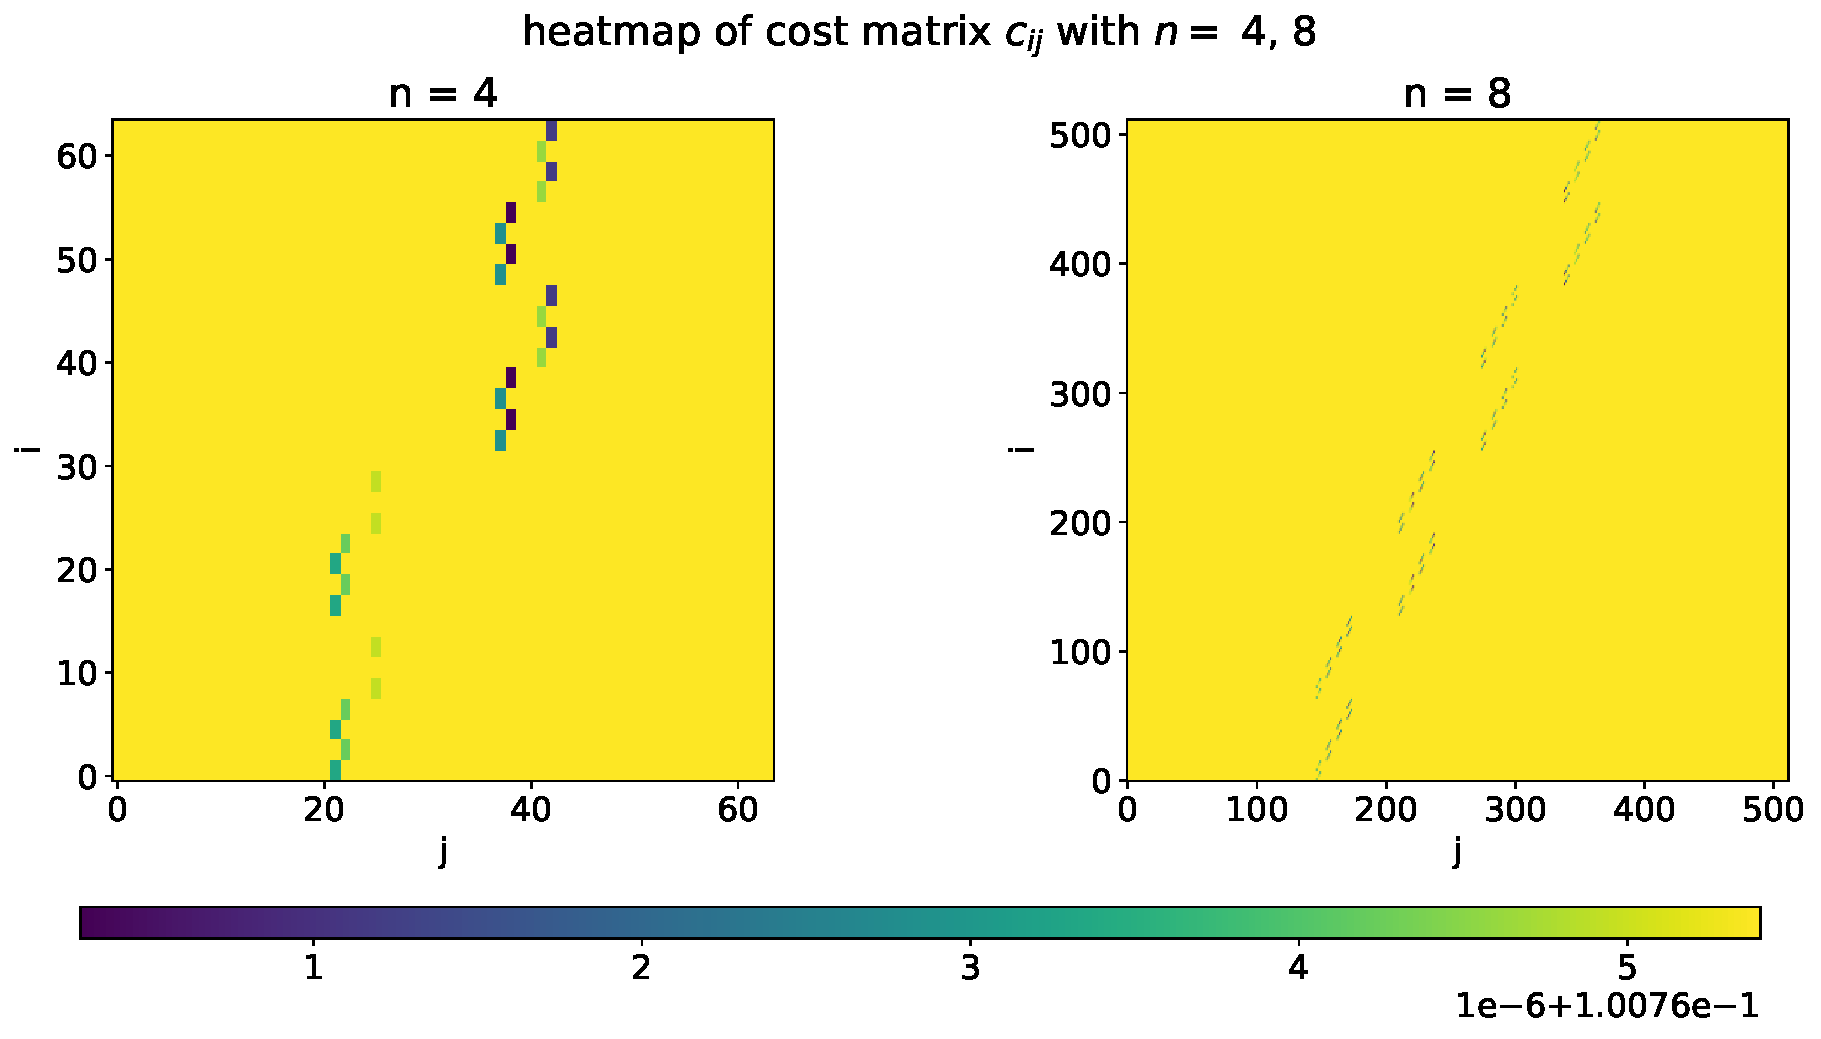
\includegraphics[width=\textwidth]{./images/uniform_collapse_ma_ncombined-n8-new.pdf}
	\caption{Heat map of the cost matrix for uniform collapse, for $n = 4$ (left) and $n = 8$ (right), as retrieved from Algorithm~\ref{alg:1}.}
	\label{fig:unifcoll}
\end{figure}

\begin{figure}[p]
	\centering 
	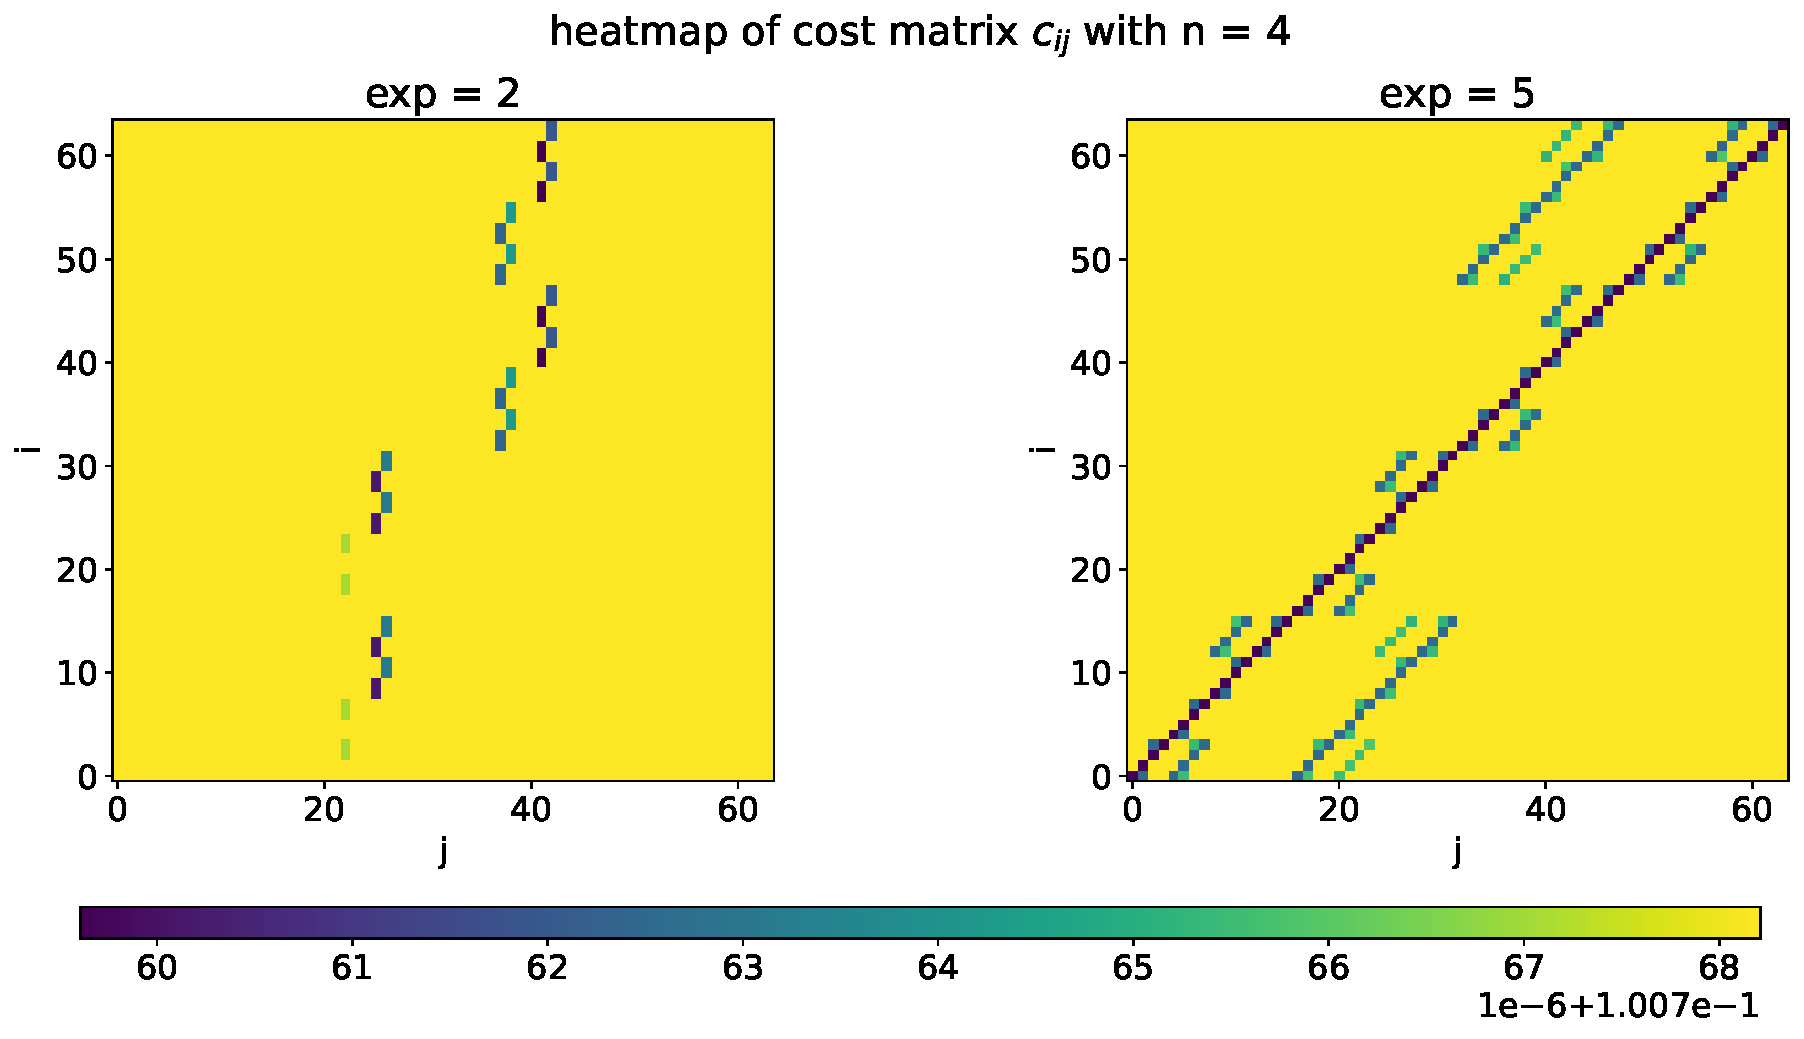
\includegraphics[width=\textwidth]{./images/nonuniform_collapse_ma_n4_c-combined-exp[2, 5]-new.pdf}
	\caption{Heat map of the cost matrix for non-uniform collapse, for both \lstinline|exp| $=2$ (left) and \lstinline|exp| $=5$ (right), for $n = 4$, as retrieved from Algorithm~\ref{alg:1}. }
	\label{fig:nonuniformcolln4}
\end{figure}

For uniform collapse, we can see for the case $n=4$, in Figure~\ref{fig:unifcoll}, what looks like a $90$ degree rotation of the cost matrix with respect to the uniform expansion case, in Figure~\ref{fig:uniformexp}. This is to be expected, as if we time-invert the expansion, we get a collapse process. Thus, you would expect $\pihat^c_{ij} = \pihat^e_{ji}$, with $\pihat^c$ the transportation matrix of collapse, and $\pihat^e$ the transportation matrix of expansion. Hence, we would also expect $c^c_{ij} \approx c^e_{ji}$, again with $c^c$ the cost matrix of collapse, and $c^e$ the cost matrix of expansion. This rotation of the expansion case is indeed what we can see in Figure~\ref{fig:unifcoll}. \par 
For the $n=8$ case, also in Figure~\ref{fig:unifcoll}, we can see that the structure is quite similar to the $n=4$ case. Again, the values of where the cost is lower can be explained by counting out the boxes and seeing where we would physically expect particles to go. \par 
If we look at non-uniform collapse, we expect for lower \lstinline|exp| structures that are quite similar to those of non-uniform expansion. In Figure~\ref{fig:nonuniformcolln4} we can see the $n=4$ case for \lstinline|exp| $=2$, which looks like a $90$ degree rotation of Figure~\ref{fig:nonuniformexpn4}, the non-uniform expansion case for $n=4$ and \lstinline|exp| $=2$.  \par 
However, when we increase \lstinline|exp|, we can see different structures emerging. In Figure~\ref{fig:nonuniformcolln4}, for $n=4$ and \lstinline|exp| $=5$, a wide, more diagonal structure can be seen, clearly distinguishable from the earlier \lstinline|exp| $=2$ case. Note that in this case, the cost matrix is clearly not a rotation of the expansion cost matrix in Figure~\ref{fig:nonuniformexpn4}. This discrepancy is probably due to the fact that the process of non-uniform expansion and collapse are not time-reversible in the same way as uniform expansion and collapse. The main reason for this discrepancy could be the asymmetry that is introduced by the non-uniformity. 


\subsection{Walls}
Another common type of motion in cosmology is a combination of expansion and collapse. One example of combination of expansion and collapse is walls (or sheets). Walls are flattened, sheet-like structures that enclose the voids, and are associated with collapse along one dimension (perpendicular to the wall), and expansion along the other two dimensions (within the plane of the wall) \citep{bos2016}. Simulations were made of these walls, again with a box size of $100$ (arbitrary units), and points started in a cube centered at $(50, 50, 50)$ with sides of length $50$. Different values for \lstinline|exp| for the expansion and collapse can be taken. We chose to consider the case where \lstinline|exp| $:=$ \lstinline|exp|$_\text{collapse}$ = \lstinline|exp|$_\text{expansion}$. The cases \lstinline|exp| $=2$ and \lstinline|exp| $=5$ were studied, as can be seen in Figure~\ref{fig:wallse1} for $n=4$. \par 
In Figure~\ref{fig:wallse1}, it can be seen that the values of the cost matrix that are not $M_c$ are around the same places as in the expansion and collapse cases. However, a different structure than in the pure collapse and expansion cases can be seen, with less values not equal to $M_c$. Because the initial condition for $n=4$ was a cube that was only in eight boxes to begin, box 21, 22, 25, 26, 37, 38, 41 and 42, we would only expect a non-$M_c$ cost in these boxes on the $i$-axis. This is indeed what we can see in both figures in Figure~\ref{fig:wallse1}. Then, with collapse along one dimensions, one would not expect much movement outward in the direction of this dimension, adding diagonal values to the cost matrix. However, from expansion along the other two dimensions, one would expect the particles to move towards other boxes, corresponding to the off-diagonal values. 

\begin{figure}[p]
	\centering 
	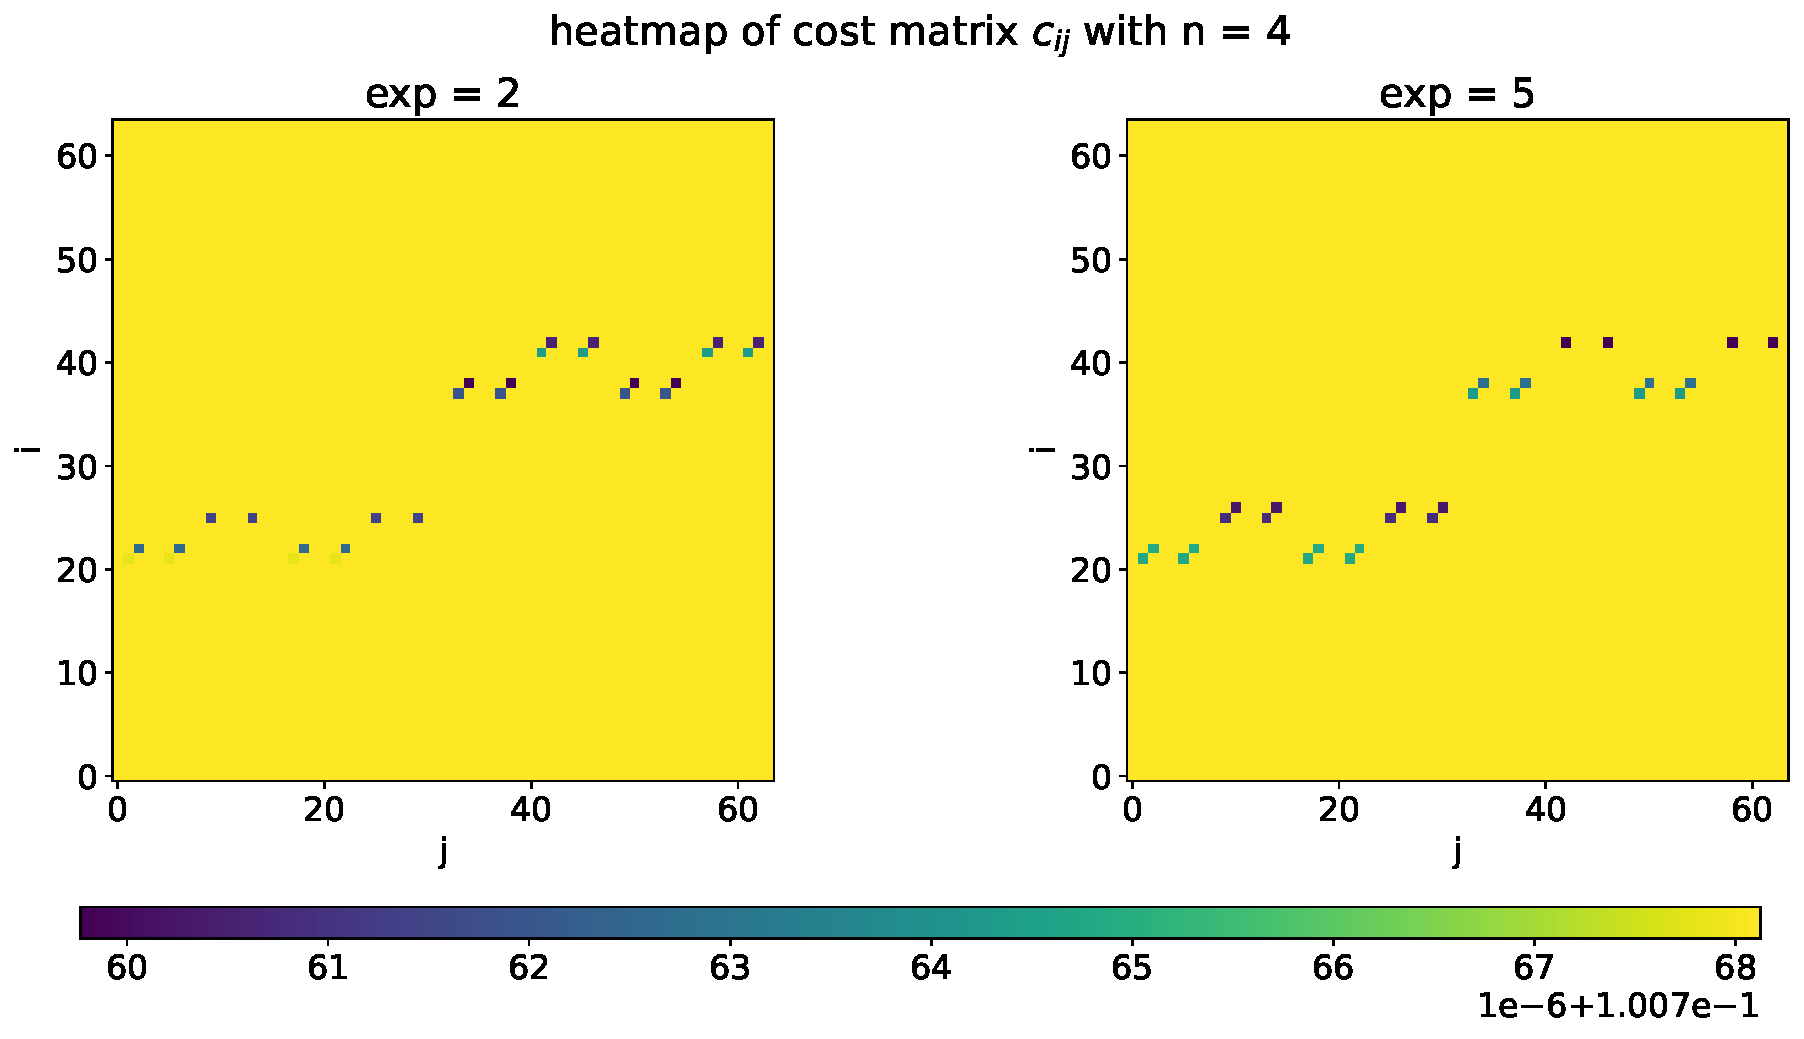
\includegraphics[width=\textwidth]{./images/walls_ma_n4_c-combined-exp[2, 5]-new.pdf}
	\caption{Heat map of the cost matrix for walls, for both \lstinline|exp| $=2$ (left) and \lstinline|exp| $=5$ (right), for $n = 4$, as retrieved from Algorithm~\ref{alg:1}. }
	\label{fig:wallse1}
\end{figure}

\begin{figure}[p]
	\centering 
	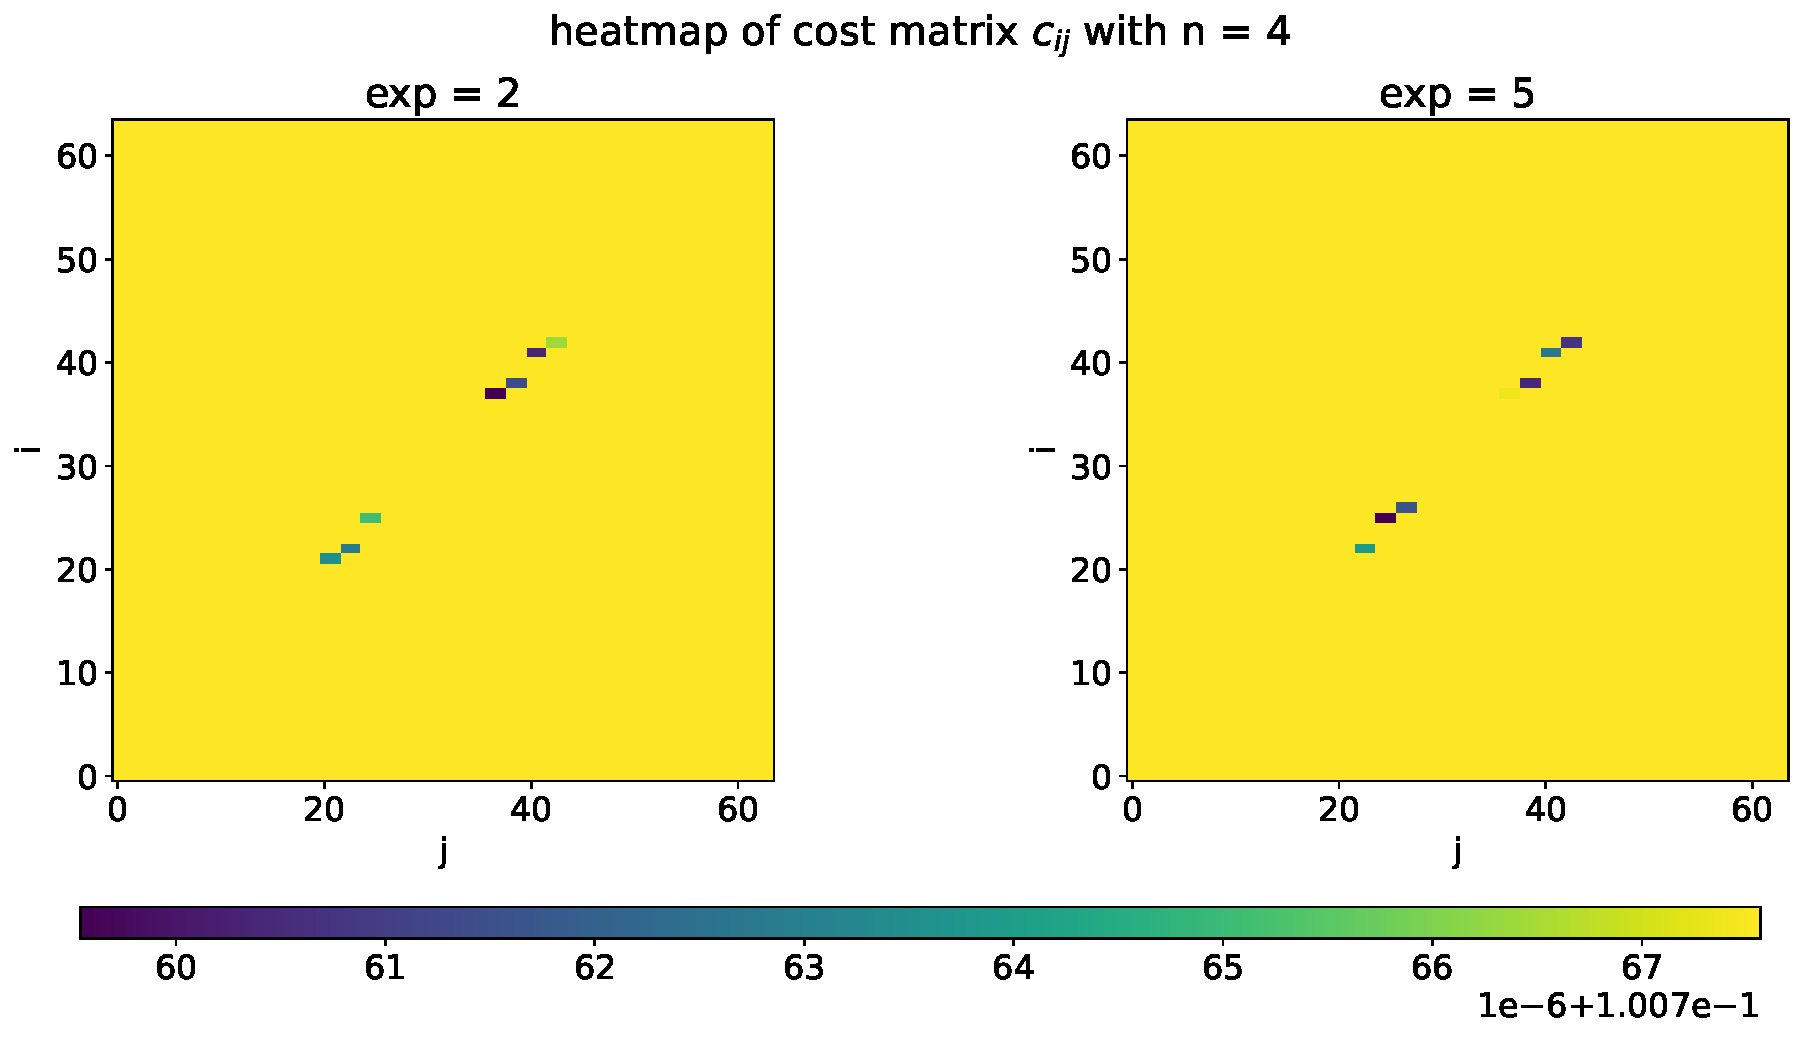
\includegraphics[width=\textwidth]{./images/filament_ma_n4_c-combined-exp[2, 5]-new.pdf}
	\caption{Heat map of the cost matrix for filaments, for both \lstinline|exp| $=2$ (left) and \lstinline|exp| $=5$ (right), for $n = 4$, as retrieved from Algorithm~\ref{alg:1}.  }
	\label{fig:filaments}
\end{figure}


\subsection{Filaments}
As a last reference case, we will look at another mixed expansion-collapse case, filaments. Filaments are associated with collapse along two dimensions (perpendicular to the filament's axis), and expansion/flow of matter along the other dimension \citep{bos2016}. We will model the latter as expansion. These simulations were made again with a box size of $100$ (arbitrary units), and points started in a cube centered at $(50, 50, 50)$ with sides of length $50$. Different values of \lstinline|exp| for the expansion and collapse can be taken. We chose, as for the walls, to consider the case where \lstinline|exp| $:=$ \lstinline|exp|$_\text{collapse}$ = \lstinline|exp|$_\text{expansion}$. Again, the cases \lstinline|exp| $=2$ and \lstinline|exp| $=5$ were studied, as can be seen in Figure~\ref{fig:filaments} for $n=4$. \par  
We can see that for $n=4$, there are very few cases where the cost matrix is not equal to $M_c$, all of which are approximately on the diagonal. This is probably due to the case that we started with a cube that was only in eight boxes to begin with, box 21, 22, 25, 26, 37, 38, 41 and 42. Therefore, on the $i$-axis, we would only expect a non-$M_c$ cost here, which is indeed what we can see in both figures in Figure~\ref{fig:filaments}. Then, with collapse along two dimensions, one would not expect much movement outward. Hence, the particles are expected to stay in, or close to, their own boxes in the $n=4$ case. 

\section{FLAMINGO Cost Matrix}
Using Algorithm~\ref{alg:1}, the cost matrix of the FLAMINGO data, as described in Chapter~\ref{ch:data}, can be found. With the reference cases described in Section~\ref{sec:refs}, we hope to interpret this cost matrix. First, we will comment on the expected cost matrix, whereafter the cost matrix as recovered from Algorithm~\ref{alg:1} will be discussed. 

\subsection{Expected Cost Matrix}
As described before in Chapter~\ref{ch:data}, the FLAMINGO simulations are hydrodynamical cosmological simulations, with the aim to understand the large-scale structure formation of the universe. Hence, knowledge about the expected large-scale structures can be used to comment on the expected cost matrix.

\subsubsection{Structure Formation in the Cosmic Web}
In large-scale structure formation, one would expect filaments, voids, sheets/walls and clusters to form, arising from the gravitational collapse of a relatively uniform initial density distribution in the early Universe. These different structures have different motions associated with them \citep{bos2016}. Voids are vast, under-dense regions, largely without many galaxies or matter. They are characterized by expansion along all three dimensions, effectively pulling matter out of the void towards the surrounding denser structures. Walls (or sheets) are flattened, sheet-like structures that enclose the voids. The walls are denser than voids, but less dense than filaments or clusters. As mentioned before, walls are associated with collapse along one dimension (perpendicular to the wall), and expansion along the other two dimensions (within the plane of the wall). Hence, matter is flowing inwards towards the central plane of the wall, while stretching out within that plane as it gets pulled towards the denser filaments and clusters. Filaments are elongated, thread-like structures. Filaments primarily have collapse along two dimensions (perpendicular to the filament's axis), and expansion/flow of matter along the other dimension. Lastly, clusters are the densest and most massive regions in the Cosmic Web. They are gravitationally bound, and therefore have (gravitational) collapse in all three dimensions. As we expect all of these cases to occur in our data, we expect the cost matrix to be some combination of these cases, and therefore a combination of our reference cases.

\subsubsection{Geodesics}
On a single-particle level, the particles are expected to take the locally shortest path between their initial and final position. Therefore, the particles are expected to move along the geodesics as recovered from General Relativity. Hence, the cost matrix is expected to comply with the laws of General Relativity and the $\Lambda$CDM paradigm, as the FLAMINGO simulations are based on these laws \citep{schaye2023}. Thus, if one were to have a very high resolution, in our case computational resolution, the problem of the search for a cost matrix could be stated in a way to be a test of General Relativity. If one were to observe particle motion in larger-scale structures in the real universe and find a cost matrix from those movements, one could check the observed cost matrix against the theoretical cost matrices from the simulations. With this comparison, one could possibly infer the cosmological parameters. However, this goes beyond the scope of this thesis, so we will not discuss it any further. 

\subsection{Recovered Cost Matrix}
With the knowledge of what we expect for the cost matrix in mind, Algorithm~\ref{alg:1} can be implemented the same way as for the reference cases in Section~\ref{sec:refs} to find the cost matrix of the FLAMINGO data. The results can be seen in Figure~\ref{fig:data}, scaled in the same was as described in Section~\ref{sec:refs}. For the $n=4$ case, in Figure~\ref{fig:datan4}, we can already see that the structure of the cost matrix is more complicated than the previous reference cases, which is what is to be expected. It is expected that there is quite a lot of local collapse and expansion going on, in contrast to the only one scale of expansion and collapse in the reference cases. However, this makes it difficult to interpret the cost matrix on first sight. \par 
For $n=8$, in Figure~\ref{fig:datan8}, the cost matrix looks quite similar to the $n=4$ case, still with the diagonal stripes. However, it is also clear that this is quite far from any reference case in Section~\ref{sec:refs}. \par 

\begin{figure}[p]
	\centering
	\subfloat[Cost matrix with $n=4$.]{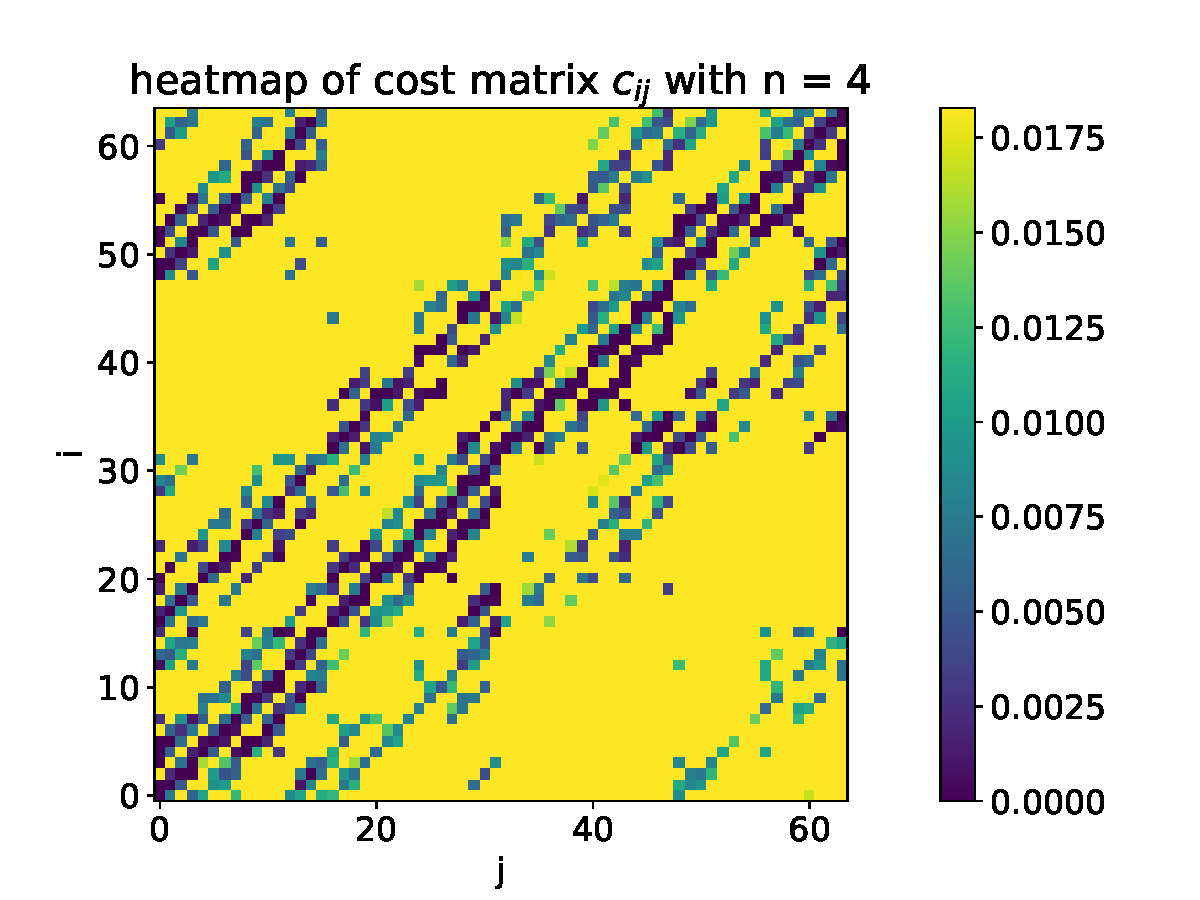
\includegraphics[width=0.8\textwidth]{./images/c-n4-new-zeros.pdf}\label{fig:datan4}}
	\\
	\subfloat[Cost matrix with $n=8$.]{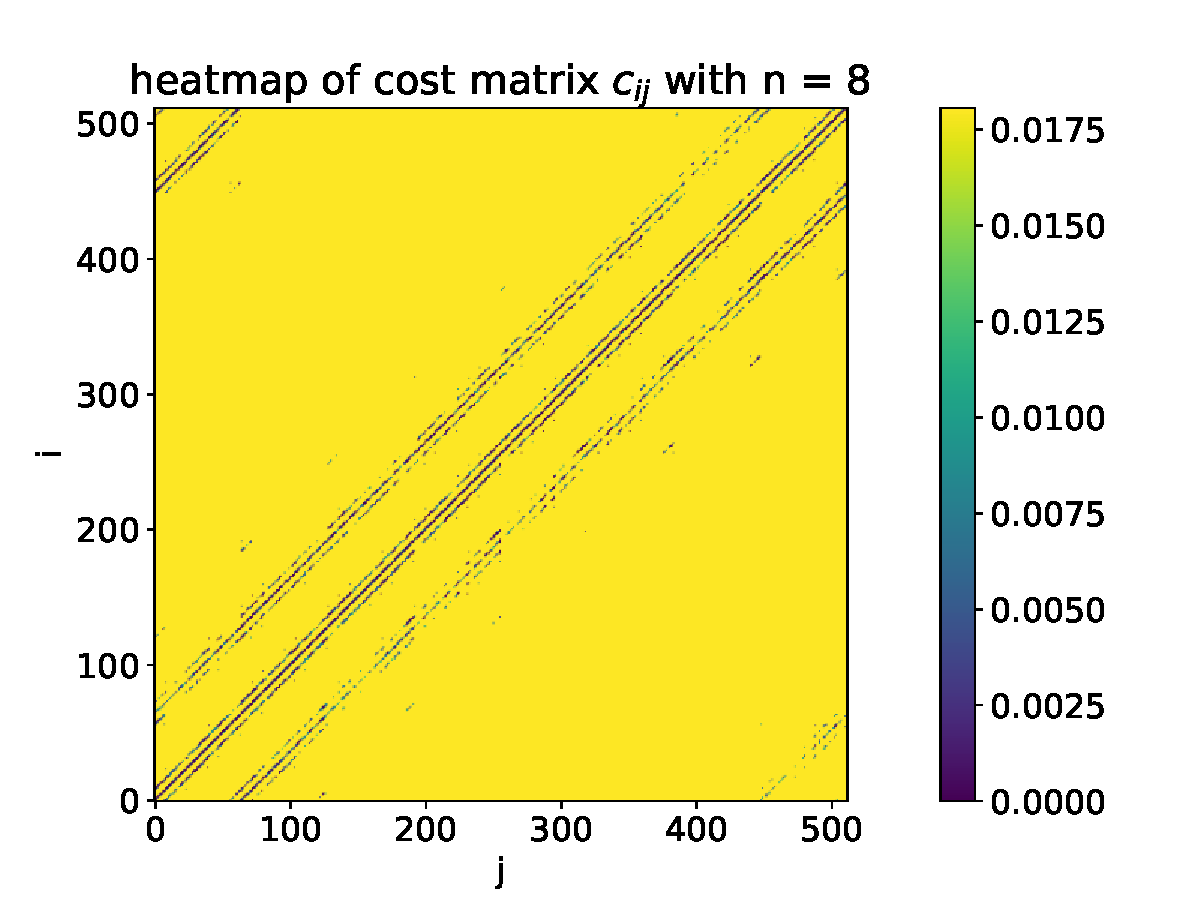
\includegraphics[width=0.8\textwidth]{./images/c-n8-new-zeros.pdf}\label{fig:datan8}}
	\caption{Heat map of the cost matrix for the FLAMINGO data, for $n = 4$ and $n = 8$, as retrieved from Algorithm~\ref{alg:1}.}
	\label{fig:data}
\end{figure}

As touched on before, it is expected that there is a lot of different kinds of motion going on in the simulation, and it is difficult to visually distinguish the different motions from these cost matrices. Note, however, that both cost matrices in Figure~\ref{fig:data} look quite symmetric, which implies isotropy and is what is to be expected from the cosmological principle.

\subsection{Markov Chain Monte Carlo Simulation} 
One way to interpret these results is through the assumption that the FLAMINGO results are a linear combination of multiple different reference cases. \par 
To test this assumption, simulations of more reference cases were done, without the simulation necessarily filling the whole box. For better computational efficiency, $500$ thousand particles were simulated instead of $1$ million as in Section~\ref{sec:refs}. Particles were simulated to expand from a cube of length $50$ (arbitrary units) to a cube of length $100$, or to collapse from a cube of length $100$ to a cube of length $50$. The box size was chosen to be $400$. Multiple centers for the expansion were chosen: $(x, y, z)$ with $x, y, z \in \{100, 200, 300\}$, as well as multiple values of \lstinline|exp|, \lstinline|exp| $\in \{0.4, 1, 2, 5\}$. With this, $27$ reference cases for each type of motion were made, all with $4$ \lstinline|exp| values, and both for expansion and collapse. This resulted in 216 reference cases. However, it is expected that this is not enough, as there is only expansion and collapse possible from a limited number of points in the box. \par 
As a proof of concept to test the hypothesis that the FLAMINGO cost matrix is a linear combination of the reference cases, a Markov Chains Monte Carlo (MCMC) simulation was used. For MCMC, one needs to consider Bayes' formula \citep{grimmett2014}: 
\begin{equation}
	\P(A|B) \propto \P(B|A) \P(A),
\end{equation}
with $\P(A|B)$ the posterior probability, $\P(B|A)$ the likelihood and $\P(A)$ the prior. Here, $A$ can be seen as the model, and $B$ as the data. A Gaussian prior was used, 
\begin{equation}
	\P(A) = \prod_i e^{-(\theta_i - \hat{\theta}_i)^2/2\sigma_i^2},
\end{equation}
with $\theta$ a vector of model parameters, $\hat{\theta}_i$ the initial guess for parameter $\theta_i$, and $\sigma_i$ the width of the prior. Note that $\sigma_i$ should be large enough to allow the model to move away from the initial guess $\hat{\theta}$, but not so large that it jumps into regions deemed unrealistic and therefore having a higher computational cost then necessary. To ensure numerical stability, a simple bound that returns negative infinity if any of the input elements were bigger than some limit was added to this Gaussian prior, where we used a limit value of $1000$. A similar bound on the parameter values was implemented to ensure all parameters are non-negative. For the likelihood, a Gaussian was also used. For all $\sigma_i$, a value of $0.5$ was used. \par 
The Python library \lstinline|emcee| is used for the MCMC simulation \citep{emcee}. The simulation was run by 1000 walkers and 5000 steps for each walker. We will get some randomly generated, uniformly distributed starting positions, and set up and run a sampler afterwards. Then, we will need to look at the best values for the fit, and marginalize the data, using 
\begin{equation}
	P(a|B) = \int P (a,b|B) \d b,
\end{equation}
where $a$ and $b$ are parameters of the fit. The median of the distribution will be calculated as the best value, and the $16$th and $84$th percentiles as the uncertainty range. \par 
For the MCMC, we used cost matrices with $n=8$, so $8^3$ boxes. Cost matrices with $n=8$ for the reference cases are discussed in Appendix~\ref{sec:apprefs}. We can see the evolution of the walkers for the first few parameters in Figure~\ref{fig:mcmcwalkers}. \par 
\begin{figure}[p]
	\centering
	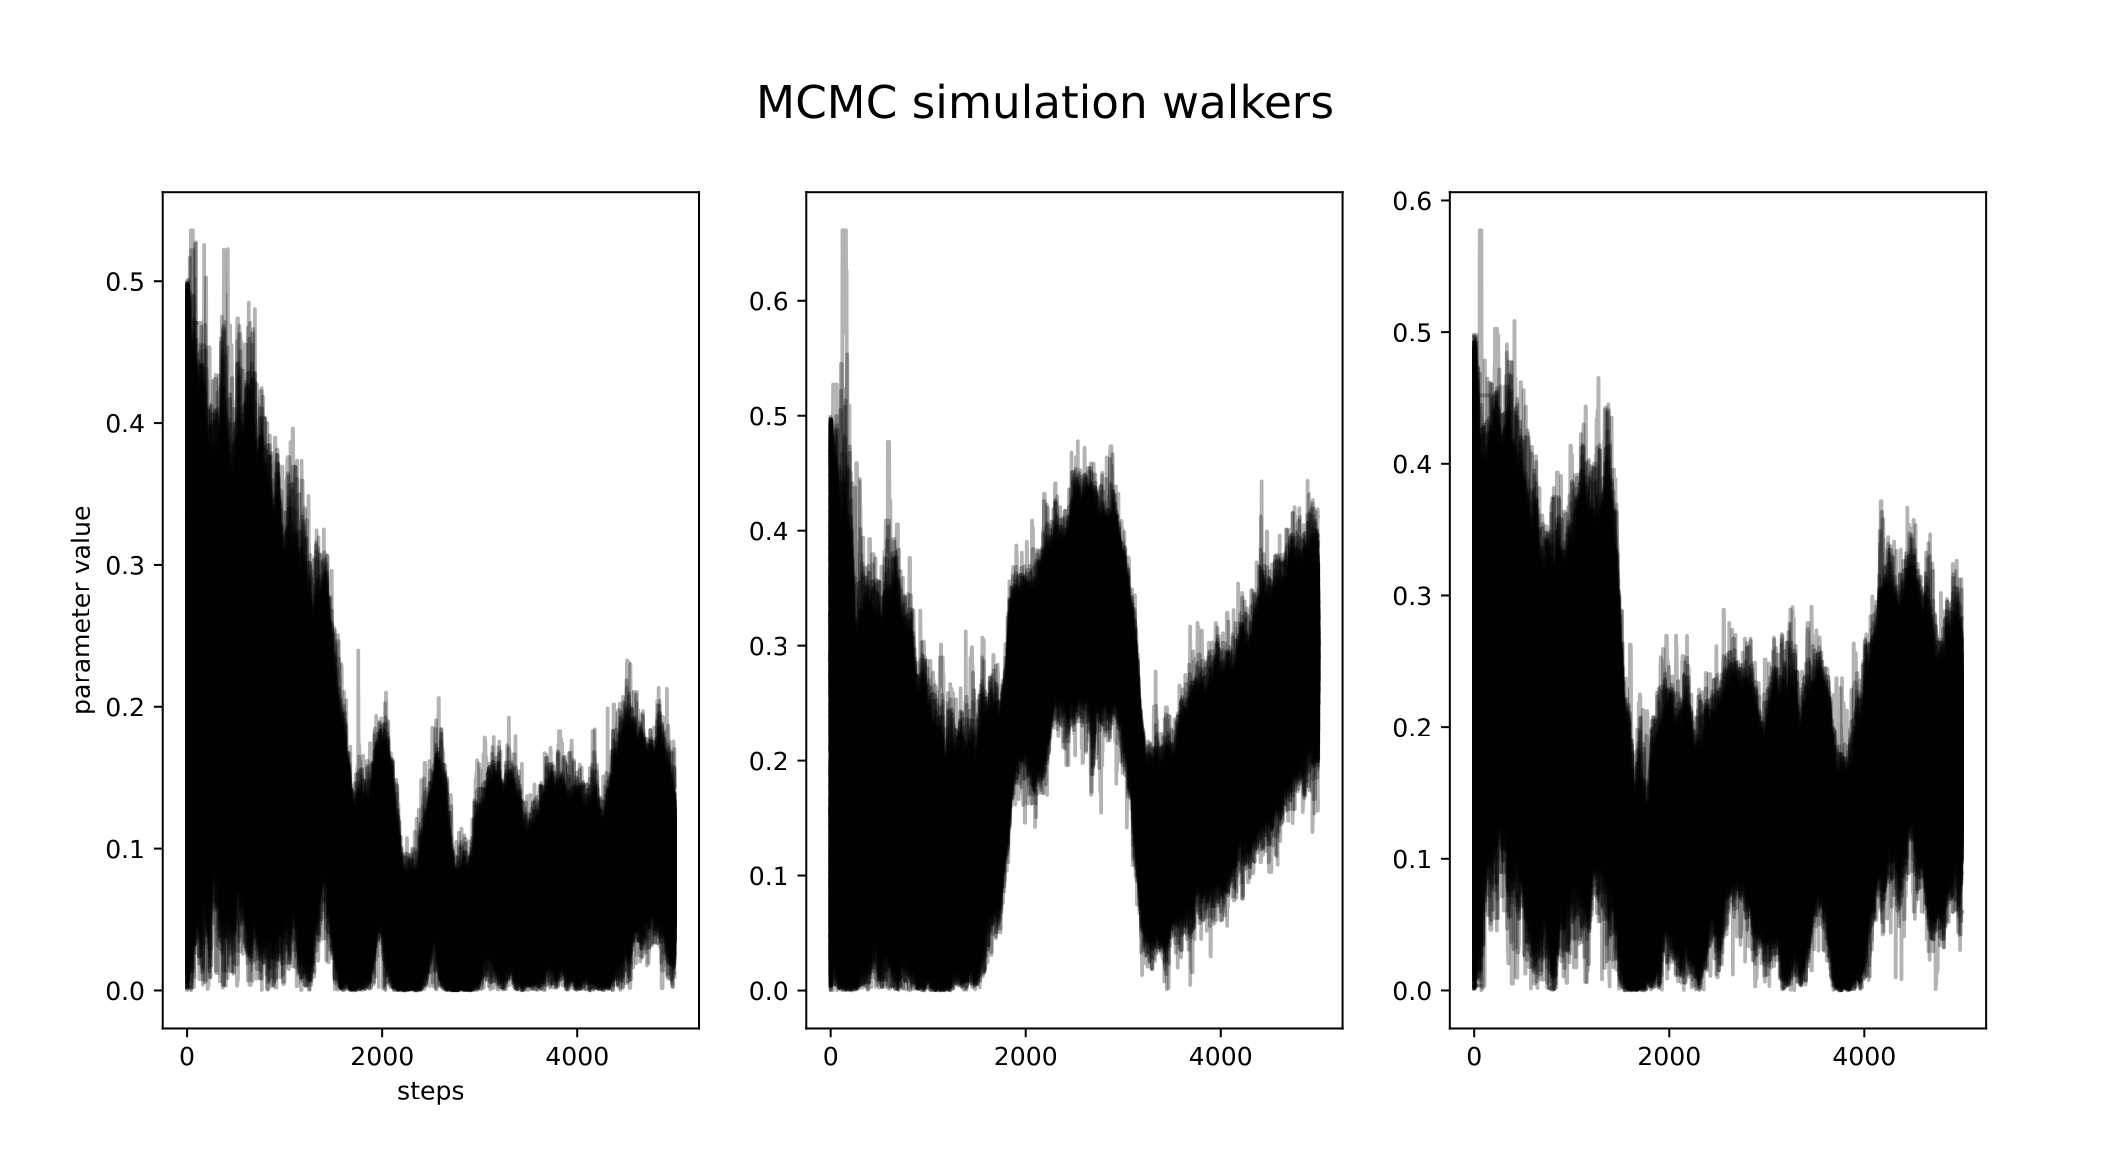
\includegraphics[width=\textwidth]{images/sampler.png}
	\caption{MCMC walkers for the first few parameters; expansion from $(100, 100, 100)$ (left), expansion from $(100, 100, 200)$ (middle) and expansion from $(100, 100, 300)$ (right).}
	\label{fig:mcmcwalkers}
\end{figure}

We can see that the chains are not converging well. This aligns with our expectation that the 216 described reference cases are not enough. The expectation is that more reference cases will solve this issue, but we cannot rule out the possibility that the FLAMINGO data is not a linear combination of the described reference cases or our initial guesses of parameters were too far off. \par 

\begin{figure}[p]
	\centering
	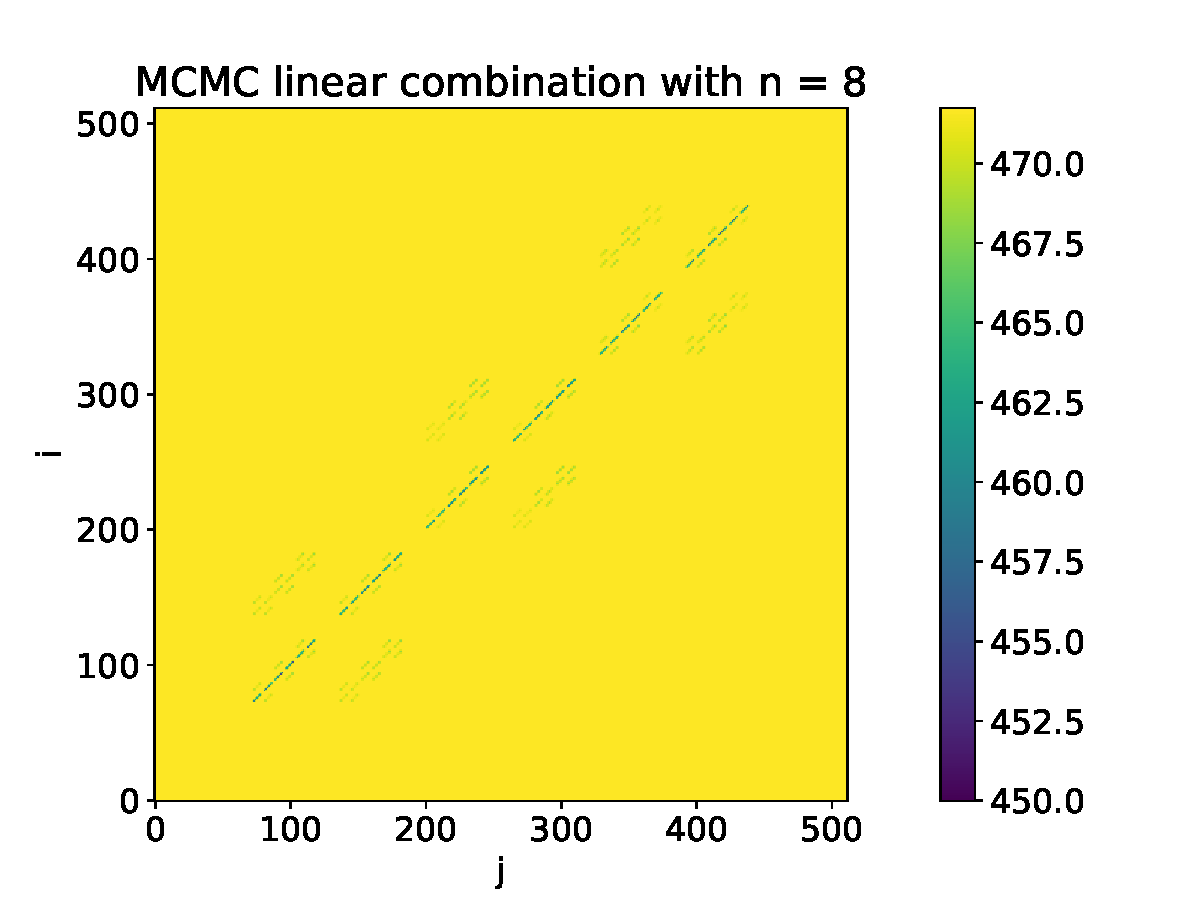
\includegraphics[width=0.8\textwidth]{images/mcmc_cost}
	\caption{Cost matrix from the linear combination of the MCMC, with $n=8$.}
	\label{fig:mcmccost}
\end{figure}

The cost matrix from these MCMC results can be seen in Figure~\ref{fig:mcmccost}. As described before, the median value is used as best-fit parameter. It can be seen that the values of this cost matrix are indeed far off from the FLAMINGO data, in Figure~\ref{fig:data}. \par 
To better show how far off this cost matrix is, the differences between the FLAMINGO cost matrix and the cost matrix from the linear combination of the MCMC can be seen in Figure~\ref{fig:mcmcdiffs}. It is clear that the MCMC fit is not a good fit and does not describe the data well. 


\begin{figure}[!ht]
	\centering
	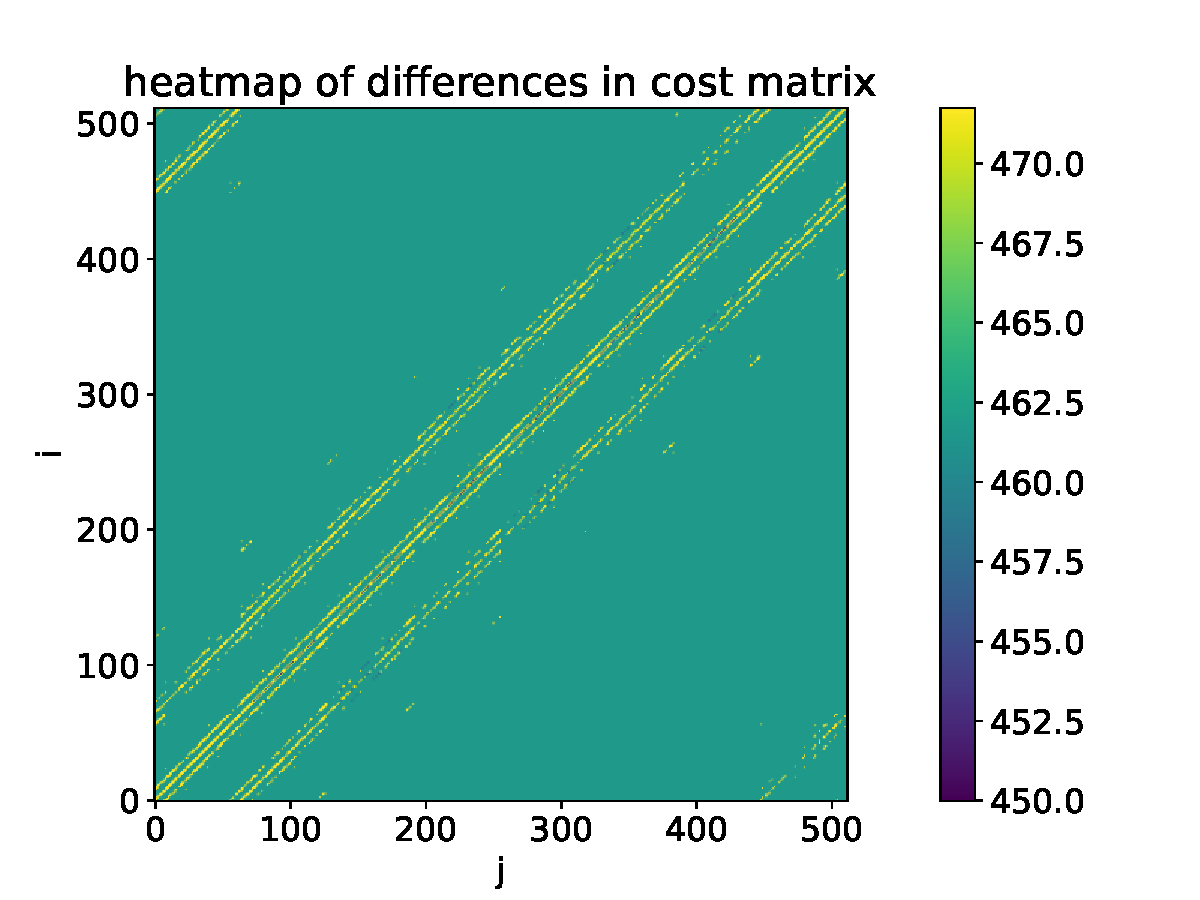
\includegraphics[width=0.8\textwidth]{./images/costmatrix-mcmc-diff.pdf}
	\caption{Differences between the FLAMINGO cost matrix and the cost matrix from the linear combination of the MCMC, for $n=8$.}
	\label{fig:mcmcdiffs}
\end{figure}

















